\section{Introduction}
\label{sec:intro}

%The nearest neighbors (NN) search problem aims to find objects that are close to the given query, which is the basic and important problem in a wide range of applications, such as artificial intelligence, pattern recognition, information retrieval and so on. However, as the dimensionality of data objects increases, the performance of most existing methods \cite{kdtree,rtree,srtree} for exact NN search degenerates or be even worse than the brute-force linear-scan approach \cite{linscan}. Due to the difficulty in finding an efficient method for exact NN search in high-dimensional space, many researchers have focused on approximate nearest neighbors search as an alternative approach.

The nearest neighbors (NN) search problem aims to find objects that are close to the given query, which is the basic and important problem in a wide range of applications. Due to the difficulty in finding an efficient method for exact NN search in high-dimensional space, many researchers have focused on approximate nearest neighbors search as an alternative approach. Locality sensitive hashing (LSH) \cite{orilsh} is known as one of the most promising indexing methods for approximate nearest neighbors search, where the locality sensitive hash function has the property that points that are closer to each other have a higher probability of colliding than points that are farther apart.

%To improve the hashing effect, $m$ randomly chosen LSH functions are utilized together to generate a compound hash key for each object $o$. In compensation for the loss of candidate points because of importing compound hash key, a large number $l$ of hash tables are constructed.

\begin{comment}
\begin{figure}[t]
    \centerline{\includegraphics[width=2.8in]{fig/density_color.eps}}
    \caption{The distribution of point densities (KDD dataset).}
    \label{fig:density_query}
\end{figure}
\end{comment}


Many LSH variants are proposed in recent years. From the index structure's point of view, these LSH variants can be classified into two categories, \emph{\textbf{table-based}} index \cite{Panigrahy:2006:EBN:1109557.1109688, mplsh,c2lsh,Haghani:2009:DSS:1516360.1516446,Huang:2015:QLH:2850469.2850470,Zheng:2016:LAN:2882903.2882930} and \emph{\textbf{tree-based}} index \cite{lsb,sklsh,Bawa:2005:LFS:1060745.1060840}. E2LSH \cite{datar} is a typical table-based LSH which proposes a hash function used in Euclidean space. The data points with the same hash value or the same concatenating hash values are placed in the same bucket, which implies that they are close to each other. The approximate NN search is achieved by returning the data in the same bucket as which the query falls in. Different from the intuitive table-based LSH structures, another set of LSH variants exploit tree structures. LSB \cite{lsb} and SK-LSH \cite{sklsh} share the similar idea that projects high-dimensional objects to a sequence of one-dimensional sortable values (e.g., $z$-value in LSB or compound hash key in SK-LSH), such that the linear order preserves the similarities between any two objects. The sequence of ordered values are then indexed by a B-tree like structure, and the NN search can be achieved by a bi-directional expansion process started from the B-tree node that corresponds to the query.

%All the previous research efforts have improved the basic LSH a lot on both efficiency and effectiveness.


%Datar et al. propose the hash function used in Euclidean space \cite{datar}, and its open-source implementation E2LSH package\footnote{http://www.mit.edu/~andoni/LSH/} has been widely used. In this paper, we will focus on the LSH in Euclidean space and the E2LSH index structure. Multi-probe LSH \cite{mplsh} is inspired by and improve upon entropy-based LSH \cite{Panigrahy:2006:EBN:1109557.1109688}, which can find similar objects from a single or small number of hash tables by exploring the buckets ``near'' the one where the query falls.

%C2LSH, QALSH, DSH, selective lsh, LasyLSH[sigmod 2016] Accelerating Large Scale Centroid-based Clustering with Locality Sensitive Hashing [ICDE 2016]
\begin{figure}[!t]
\vspace{-0.1in}
	\centerline{\subfloat[LSH]{\includegraphics[angle=-90, width=1.8in]{fig/lsh_kdd_density.eps}
    \label{fig:densdist:lsh}}
    \hspace{-0.1in}
    \subfloat[LSB]{\includegraphics[angle=-90,width=1.8in]{fig/lsb_kdd_density.eps}
    \label{fig:densdist:lsb}}
    }
    \vspace{-0.1in}
	\caption{The density of hash values for KDD dataset (in log scale). Each bar in LSH represents the number of points in a bucket, while in LSB represents the number of points in a $z$-value range.}
	\label{fig:densitydist}
\vspace{-0.2in}
\end{figure}


However, most of these LSH index structures fail to take data distribution into account. They perform well in a uniform data distribution setting, but exhibit instable performance when the data are skewed. As known, most real life data are skewed, which makes LSH suffer. Based on our observation, the skewed data distribution leads to skewed hash values, and the skewness of hash values is the potential reason for the performance degradation. The Euclidean-based LSH function \cite{datar} projects high-dimensional data points to a real number line and partitions the line into fixed-length intervals. As a result, the hash values exhibit skewed distribution as long as the original data are skewed. The points with the same hash values are assigned to the same bucket, so the bucket sizes vary greatly. Figure \ref{fig:densdist:lsh} shows the skewed bucket size distribution for the KDD dataset (Table \ref{tab:data}). Intuitively, LSH-based $k$NN search displays higher accuracy for dense queries\footnote{A query falling in a dense bucket/range is referred to as a dense query, and vice versa.} while lower accuracy for sparse queries. This is because the distances from query $q$ to its $k$NNs are small (or large) in a dense (or sparse) region, so that they are likely (or unlikely) to be hashed to the same bucket. On the other hand, due to the large bucket size, it displays higher cost (evaluated by the number of distance measurements) for dense queries than sparse queries. This phenomenon is illustrated in Figure \ref{fig:dens:lsh}. %Multi-probe LSH (mplsh) \cite{mplsh} improves the accuracy of sparse queries by searching nearby buckets but still requires higher cost for dense queries.

For another type of LSH index structures, tree-based LSH indices, the approximation accuracy and cost are also related to the density of hash values. As a representative tree-based LSH index structure, LSB \cite{lsb} hashes the data points to the sortable one-dimensional $z$-values and maintains them with a B-tree like structure. Figure \ref{fig:densdist:lsb} shows the histogram of hash values (i.e., $z$-values) for the KDD dataset. We can see skewed $z$-values distribution. When performing different types of queries on the LSB-tree, as shown in Figure \ref{fig:dens:lsb}, it displays higher accuracy for sparse queries but lower accuracy for dense queries. The reason can be explained as follows. A query in dense range has smaller distances to its $k$NNs. If the returned approximate $k$NNs are far apart from the query, it will incur remarkable diversity of the distances to its real $k$NNs, so that the accuracy will be seriously impacted. Unfortunately, by using $z$-values the spatial locality is not always preserved as pointed out in \cite{zorkderknn} and \cite{Zhang:2012:EPK:2247596.2247602}, it indeed returns far apart points sometimes. This approximation error is even amplified for dense queries, so the dense queries suffer from the low accuracy problem.


\begin{figure}[!t]
\vspace{-0.2in}
	\centerline{\subfloat[LSH]{\includegraphics[angle=-90, width=1.8in]{fig/lsh_ratio.eps}
    \label{fig:dens:lsh}}
    \hspace{-0.1in}
    \subfloat[LSB]{\includegraphics[angle=-90,width=1.8in]{fig/lsb_ratio.eps}
    \label{fig:dens:lsb}}
    }
    \vspace{-0.1in}
	\caption{Density of hash values vs. query accuracy and query cost (KDD). Smaller error ratio indicates higher accuracy, which is defined in Equation (\ref{eq:ratio}).}
	\label{fig:lshdens}
\vspace{-0.in}
\end{figure}


%As known, the real world datasets exhibit non-uniform distribution property. Unfortunately, the basic LSH partitions the high-dimensional space uniformly. This may result in unbalanced hash buckets (partitions) as illustrated in Figure \ref{fig:partition:lsh}. If a hash bucket is light loaded, some existing LSH variants (e.g., \cite{mplsh,entropy}) could be used to search nearby buckets. However, if a hash bucket is heavy loaded, the large amount of distance measurements will make the approximation less effective since all the objects in that bucket are required to be examined. This terrible ineffectiveness is even worse for approximate complete NN join, since the complexity is quadratic to the bucket size. Although the partition granularity can be controlled by tuning the LSH partition width parameter, partitions of a non-uniform distributed dataset are still unbalanced.

In this paper, we propose to rebuild LSH index structures by exploring the density of hash values. The hash values in dense ranges are rehashed to make them distributed more evenly, so as to reduce the query cost. The hash values in sparse ranges are merged to be returned together during query processing, so as to improve the search quality. Therefore, the rebuilt LSH indices become more targeted in terms of data distribution. By carefully choosing the number of groups and hash functions for rehashing, the search quality can still be guaranteed.

%Since the rehashing process might be executed recursively, the newly reconstructed LSH index can be a multi-layered structure.

%But the idea can be applied to many other LSH variants.

\Paragraph{Difference to Data Sensitive Hashing} The recently proposed data sensitive hashing, e.g., DSH \cite{Gao:2014:DDS:2588555.2588565} and selective hashing \cite{Gao:2015:SHC:2783258.2783284}, also leverages data distributions. DSH \cite{Gao:2014:DDS:2588555.2588565} chooses the most suitable hashing family by learning data distributions. Selective hashing \cite{Gao:2015:SHC:2783258.2783284} creates multiple LSH indices with different granularities (i.e., radii) and locates each point only in one suitable LSH index according to data densities. These data sensitive hashing techniques learn the appropriate hash families from the data, and accordingly have the ability to create relatively balanced indexing structures. Our approach is orthogonal to them since we rely on the density of hash values and directly rebuild the existing index structures. Moreover, our rebuilding scheme can also be used as a postprocessing step for these data sensitive hashing techniques to further improve performance. We will rebuild DSH index to illustrate the possibility.

%a new indexing scheme, \emph{layer-LSH}, that bounds the bucket size by splitting large bucket into smaller buckets on multiple layers. After applying the basic LSH and partitioning the space on the root layer, our scheme will further split the large buckets with a finer partition width, so that a dense partition is further fined with multiple small partitions. This is illustrated in Figure \ref{fig:partition:layerlsh}. To achieve the same success probability (reduce false positives), multiple finer partitions of the same subspace are required. This process proceeds recursively until all the buckets are small enough, i.e., multiple LSH layers could exist.

%\setlist[itemize]{leftmargin=*}
\Paragraph{Contributions} We list our contributions as follows.
\begin{itemize}[leftmargin=*]
\item We rebuild the basic LSH structure and design \textbf{LayerLSH} (Section \ref{sec:reclsh}). The points in overloaded bucket are recursively rehashed to multiple groups of smaller buckets, forming a multi-layered index structure. Thus, the query is more efficient since a less number of more accurate NN candidates are returned. Further, by carefully choosing the new set of rehashing LSH parameters, the collision probability can be guaranteed. We also propose a stream processing approach to adapt streaming data.
\item To demonstrate the applicability to other LSH variants, we also rebuild a tree-based LSH index LSB and a data-sensitive hash index DSH, and propose \textbf{LayerLSB} and \textbf{LayerDSH} (Section \ref{sec:extension}).
  %\item We rebuild LSB structure and design \textbf{LayerLSB} (Section \ref{sec:reclsb}). The $z$-values in dense ranges are recursively rehashed in multiple child trees, which forms a multi-layered tree structure. Since extra efforts are put into indexing the dense points, the search quality is improved. Further, with consistent parameters setting, the theoretical guarantee of quality can still be guaranteed.
\item We conduct extensive experiments on real datasets to verify the effectiveness and efficiency of the proposed multi-layered structures. LayerLSH can reach the same search quality as LSH with only 5\%-20\% query cost. LayerLSH also exhibits much better performance on distributed point density approximation (Section \ref{sec:expr}).
\end{itemize}

%We survey the related work in Section \ref{sec:related}. Finally, we conclude our work in Section \ref{sec:conclusion}.
